\documentclass[a4paper,8pt]{article}
\usepackage{ifsym}
\usepackage{graphicx}
\usepackage{marvosym}
\usepackage{amsmath, amssymb, hyperref, enumitem}
\usepackage{fontspec} 	
%for loading fonts
\usepackage{capt-of}
\usepackage{xunicode,xltxtra,url,parskip} 	%other packages for formatting
\RequirePackage{color,graphicx}
\usepackage[usenames,dvipsnames]{xcolor}
\usepackage[big]{layaureo} 				%better formatting of the A4 page
% an alternative to Layaureo can be ** \usepackage{fullpage} **
\usepackage{supertabular} 				%for Grades
\usepackage{titlesec}					%custom \section
\usepackage{fontawesome}
%Setup hyperref package, and colours for links
\usepackage{hyperref}
\definecolor{linkcolour}{rgb}{0,0.2,0.6}
\hypersetup{colorlinks,breaklinks,urlcolor=linkcolour, linkcolor=linkcolour}

%FONTS
\defaultfontfeatures{Mapping=tex-text}
%\setmainfont[SmallCapsFont = Fontin SmallCaps]{Fontin}
%%% modified for Karol Kozioł for ShareLaTeX use
\setmainfont[
SmallCapsFont = Fontin-SmallCaps.otf,
BoldFont = Fontin-Bold.otf,
ItalicFont = Fontin-Italic.otf
]
{Fontin.otf}
%%%


%CV Sections inspired by: 
%http://stefano.italians.nl/archives/26
\titleformat{\section}{\Large\scshape\raggedright}{}{0em}{}[\titlerule]
\titlespacing{\section}{0pt}{3pt}{3pt}
%Tweak a bit the top margin
%\addtolength{\voffset}{-1.3cm}

\hyphenation{im-pre-se}

%-------------WATERMARK TEST [**not part of a CV**]---------------
\usepackage[absolute]{textpos}

\setlength{\TPHorizModule}{30mm}
\setlength{\TPVertModule}{\TPHorizModule}
\textblockorigin{2mm}{0.65\paperheight}
\setlength{\parindent}{0pt}

\def\house{\hbox{\kern3pt \vbox to13pt{}% 
   \pdfliteral{q 0 0 m 0 5 l 5 10 l 10 5 l 10 0 l 7 0 l 7 5 l 3 5 l 3 0 l f
               1 j 1 J -2 5 m 5 12 l 12 5 l S Q }%
   \kern 13pt}}

%--------------------BEGIN DOCUMENT----------------------
\renewcommand{\labelitemi}{$\circ$}
\begin{document}

%WATERMARK TEST [**not part of a CV**]---------------
%\font\wm=''Baskerville:color=787878'' at 8pt
%\font\wmweb=''Baskerville:color=FF1493'' at 8pt
%{\wm 
%	\begin{textblock}{1}(0,0)
%		\rotatebox{-90}{\parbox{500mm}{
%			Typeset by Alessandro Plasmati with \XeTeX\  \today\ for 
%			{\wmweb \href{http://www.aleplasmati.comuv.com}{aleplasmati.comuv.com}}
%		}
%	}
%	\end{textblock}
%}

\pagestyle{empty} % non-numbered pages

\font\fb=''[cmr10]'' %for use with \LaTeX command

%--------------------TITLE-------------
\begin{center}
{\Huge Casper Dani\"{e}l Dijkstra}
\end{center}
\begin{minipage}{0.75\textwidth}
%\par{\centering
		{\small \begin{tabular}{rl}

    \faGithub & \href{https://github.com/cdijkstra}{github.com/cdijkstra} \\
    \faLinkedin & \href{https://www.linkedin.com/in/casper-dijkstra-30661897}{https://www.linkedin.com/in/casper-dijkstra} \\
     \textifsymbol{18} & Beneluxlaan 128, \\ 
    & Utrecht, the Netherlands\\
     \Mobilefone   & 0636335440\\
      \Letter   & \email{casperdijkstra92@gmail.com} & \\
\end{tabular}
	}
%\bigskip\par}
\end{minipage}
\begin{minipage}{0.25\textwidth}
%\vspace{1.5mm}
%\centering
\hspace*{-2.35cm}
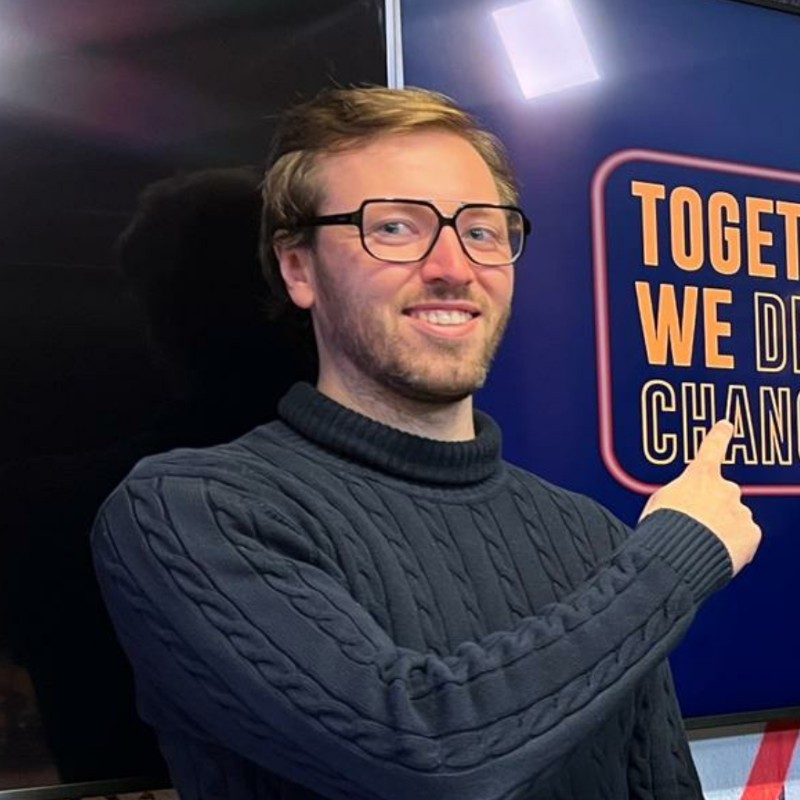
\includegraphics[width=0.85\textwidth]{casper.jpg}
\end{minipage}

%--------------------SECTIONS-----------------------------------
%Section: Personal Data
\section{Introduction}
Complex problems that require both abstract and creative problem-solving skills are what I love to work on. Especially the kind of problems that make the world a more sustainable, enjoyable, or affordable place. My unique skillset involves .NET software development and Microsoft Azure but also mathematics and philosophy. I have 7 years of experience as a software developer with different codebases and am knowledgeable about the features that Azure provides to run robust and highly available applications. 

\noindent
Besides hard skills I have developed invaluable soft skills including good collaboration skills (e.g. updating about the progress of PBIs, or asking for help if needed), staying calm when deadlines approach and am usually described as a very sociable and humorous person. I thrive in creative environments where knowledge-sharing is encouraged, challenging puzzles have to be solved that require critical thinking, and with a nonhierarchical people-centric culture. 

\section{Work Experience}
\textbf{Azure Cloud Engineer and Linux Engineer} (June 2024 - December 2024) \\
Hogeschool van Amsterdam (Amsterdam), via \textbf{Freshminds} (Leiden) \\
I migrated the OTAP environments of the main website of the applied university to secure Azure subscriptions, 
 where management group policies are enforced, and no Azure Policy warnings remain.
 This ensured the website is future-proof,
deployments can be rolled out through a Gitlab CI / CD street, and reduced the monthly cloud expenditure of the team by 55\%. \\
\textit{Responsibilities \& Achievements}
\begin{itemize}
\item Migrate and harden cloud components to a Hub spoke architecture with company policies enabled and modifications only allowed through pipeline deployments.
\item Reduce the monthly cloud expenditure by 55\%.
\item Ensure that databases can be recovered with a 12 hour recovery period.
\item While on-prem Linux servers still receive Bloomreach traffic, ensure that they are available and work appropriately.
\end{itemize}
\textit{Technologies}: Azure Storage, SQL (PostgreSQL), NOSQL (Mongo Atlas),  GraphQL, Terraform, Bash Scripting, Gitlab, CI/CD, Ansible, Jenkins, Bloomreach,
Kubernetes, Helm, GitOps (ArgoCD), Hub-spoke Architecture

\textbf{Azure Cloud Developer} (December 2023 - May 2024) \\
NS (Utrecht), via \textbf{Freshminds} (Leiden) \\
  At team Pandas, we are responsible for robust and secure data storage at NS,
  and sharing data among data teams when allowed. I helped in constructing and maintaining a modular solution for data teams to seamlessly set up data science projects, setting appropriate permissions on projects, and enabling teams to use Terraform and Azure Devops efficiently.
  \textit{Responsibilities \& Achievements}
  \begin{itemize}
    \item Implement C\# TUI Application to simplify code changes, auto-format and validate changes for data teams
    \item Construct a simplified architecture today through which the Snowflake permissions of teams can be simplified, unified, and are protected by pull-request validations to ensure company compliance is attained.
    \item Help data teams solve their storage- and permission-related issues through ServiceNow. The questions are either conceptual or require aid with respect to pull request.
  \end{itemize}
\textit{Technologies}: Azure Storage (Storage Account, ADLS), .NET 8, Snowflake, Terraform, Python Scripting, Azure Pipelines, ServiceNow
	
\textbf{.NET Software Developer} (June 2023 - December 2023) \\
CZ (Tilburg) via \textbf{Freshminds} (Leiden) \\
I worked as full-stack software developer for health insurance CZ to develop an internal automation tool that will save the Integration Team \textasciitilde 2 days of work to publish a new service to IBM ACE by generating the required files automatically, based on the type of application and configurable parameters, in Azure Devops repositories. \\
\textit{Responsibilities \& Achievements}
\begin{itemize}
    \item Autonomously implement modular MVP application (backend and frontend) in four months.
    \item Present updates and application demo biweekly, with ensuing brainstorm session on feature request and UX improvements.
    \item Well-designed and documented APIs for all backend modules.
    \item Automated test suite for back- and frontend and CI/CD street from Azure Pipelines.
    \item Host application on private network in Azure, reachable from On-Prem network.
\end{itemize}
\textit{Technologies}: C\#, MVC, Azure, MSSQL, Bicep, JQuery, TailwindCSS, Archimate, Hub Spoke Architecture, CI/CD, Scrum, REST APIs, XML

\textbf{.NET Software Developer / DevOps Engineer} (Feb 2022 - Mar 2023) \\
\textbf{PayByLink} (Ede) via \textbf{Xebia | Xpirit} (Hilversum) \\
 I was responsible for the implementation of feature requests, operations, and implementation of quality gates, Infra-As-Code deployments, and API integrations with payment service providers.\\
\textit{Technologies}: .NET Standard, .NET Framework, Resource Files (.resx), CSS3, Javascript, Azure Function Apps, MSSQL, database migrations.


\textbf{.NET Software Developer / Azure Cloud Engineer} (Sep 2020 - Mar 2023) \\
\textbf{Taqa} (Alkmaar) via \textbf{Xebia | Xpirit} \\
 I was responsible for the configuration of a complex Kubernetes cluster, CI\/CD pipelines. 
 I also made structural changes to the Invoice service and Allocation service which calculates how much gas should flow through the gas pipeline hour by hour. I ensured that allocated quantities in the past can never change and rigorously tested these features using Specflow. \\
 \begin{itemize}
  \item 
 \end{itemize}
\textit{Technologies}: Azure (ACR, AKS, Service Bus, Defender, Storage, MSSQL, Log Analytics and more), Azure Devops, C\#,  Microservices, Event Driven Architecture, Docker, Kubernetes, High Availability with failovers, Specflow, MSTest, git, TDD. 

Cloud Engineer trainee (Aug 2020 - April 2021) \\
\textbf{Xccelerated} (Amsterdam) \\
\ \ \ Azure Cloud engineering Bootcamp for people with prior experience in software development. This involved a full-time month followed by a year with trainings on Mondays.  The rest of the week I was working at Xebia | Xpirit. \\
\textit{Technologies}: Azure architecture, Docker, Kubernetes, Terraform, Bicep, .NET, unit/integration tests

C++ Software Developer (Oct 2018 - April 2020) \\
\textbf{Rohill Engineering B.V.} (Hoogeveen) \\
\ \ \ Developed and maintained mission-critical communication products that comply with the TETRA protocol. Worked on voice-logging products, gateways and the core TetraNode solution in an agile environment. \\
\textit{Technologies}: C++, Python, Linux, UML, PostgreSQL, db failovers, SVN, Jira.

\begin{tabular}{l}	
Teacher and Summary writer (Oct 2018 - Dec 2019) \\
\textbf{AthenaStudies} (Groningen) \\
\ \ \ Help students prepare for mathematical exams by writing concise summaries and teach crash courses in: \\
\end{tabular}
\begin{itemize}[noitemsep]
    \item{} Mathematics for economics and business economics (Oct 2018)
    \item{} Mathematics and data analysis (Jan 2019)
    \item{} Matrix algebra and optimization (Dec 2019)
    \item{} Statistics II (Dec 2019)
\end{itemize}

\begin{tabular}{l}	
 Teaching Assistant (2015 - 2018) \\
 \textbf{University of Groningen} \\
\ \ \ Taught tutorials for the following courses:
 \end{tabular}
 \begin{itemize}[noitemsep]
     \item {Mechanics \& Relativity 2 (Oct 2017 - Jan 2018)
\item{} Electricity \& Magnetism 1 (Apr 2016 - July 2016)
\item{} Linear Algebra 1 (Oct 2015 - Feb 2016) 
\end{itemize}

\begin{tabular}{l}	
Practical Assistant (2013 - 2016) \\
\textbf{University of Groningen}   \\ \
\ \ \ {\small Assisted practicals for the following courses:}
\end{tabular}	
 \begin{itemize}[noitemsep]
 \item{Electricity and Magnetism 1 (3x).
 \item{Mechanics and Relativity 2 (Feb 2015 - Mar 2015).
 \item{Physics Laboratory 1 (Sep 2013 - Nov 2013).
 \end{itemize}
 
 \begin{tabular}{l}
Student Mentor (2013 - 2014) \\ 
\textbf{University of Groningen}\\
\ \ \ {\small Guided a group of first year physics students.} \\

\ \ \ {\small Informed them about university policies and career prospects as a physicist.}
\end{tabular}

\section{Programming/IT Skills}
\begin{tabular}{||p{5cm}|p{8cm}||}
\hline
Backend Programming: &  .NET (C\# 5.0+, MVC, CORE), Python, Git, Archimate \\
\hline
Frontend Programming: & HTML 5.0, CSS3, Svelte, Tailwind, Typescript, React \\
\hline
.NET:& Event Driven Architecture, Domain Driven Design, ASP.NET Identity, Microservices, Structured Logging, SignalR, Entity Framework, LINQ, Restful APIs, Razor, Blazor, XUnit, NUnit, MSTest, FluentAssertions \& Validations, SpecFlow, MOQ, Swagger, Polly, Pulumi \\
\hline
DevOps: & Azure Pipelines, Gitlab, Github Actions, CI\/CD, Git, Agile Scrum, Shell and Python scripting, SonarCloud, Whitesource, Ansible, Jenkins, IaC (Terraform, Bicep, ARM), Dashboards \\
\hline
Azure Cloud: & KeyVaults, Storage Accounts, App Services, Static Web Apps,
Managed Identity, AD Active Directory (Entra), Azure
Container Apps, ACR, AKS,
Application Insights, Log Analytics Workspaces,
SignalR, Service Bus, Event Hubs, Sendgrid, Redis,
Azure Functions, Alerts and Action Groups, Logic Apps,
SQL Server \& Elastic Pool, VNETs, Network Security Groups,
Azure AI Search (Cognitive Search), Azure OpenAI Service \\
\hline
Containerization: & Docker, Kubernetes, AKS, ACR, Container Apps \\
\hline
Databases: & MSSQL, Snowflake, PostgreSQL, MySQL, GraphQL \\
\hline
UNIX: & Command-line utilities (e.g. \verb|grep|, \verb|locate|, \verb|awk|, \verb|sed|), File System Management, Package Management, System Administration \\
\hline
Tools \& IDEs: & Jetbrain Rider, Visual Studio (Code), Vim, Nano, Postman, Slack, Teams \\
\hline
Miscellaneous: & \LaTeX \\
\hline
\end{tabular}

%Section: Scholarships and additional info
\section{Certificates and licenses}
My certificates can be found \hyperlink{https://www.credly.com/users/casper-dijkstra/badges}{here} and \hyperlink{https://learn.microsoft.com/en-us/users/casperdijkstra-0464/transcript/v2n6nap36zq90xk?tab=credentials-tab}{here}.

\begin{tabular}{l l}
HashiCorp Certified: Terraform Associate(003) & (HashiCorp, 2024) \\
AI-102: Azure AI Engineer Associate & (Microsoft, 2024) \\
AI-900: Azure AI Fundamentals & (Microsoft, 2024) \\
DP-900: Microsoft Azure Data Fundamentals  &(Microsoft, 2024) \\
Docker Certified Associate & (Docker, 2023) \\
Linux Foundation Certified Systems Administrator & (Linux Foundation, 2023) \\
CKAD: Certified Kubernetes Application Developer & (Linux Foundation, 2022) \\
CKA: Certified Kubernetes Administrator & (Linux Foundation, 2022) \\
HashiCorp Certified: Terraform Associate(002) &(HashiCorp, 2023) \\
Azure Solutions Architect Expert & (Microsoft, 2022) \\
AZ-305: Designing Microsoft Azure Infrastructure Solutions & (Microsoft, 2022) \\
AZ-500: Azure Security Engineer Associate & (Microsoft, 2022) \\
AZ-104 Microsoft Certified: Azure Developer Associate & (Microsoft, 2021) \\
AZ-204: Azure Administrator Associate certification & (Microsoft, 2021) \\
Microsoft Certified: DevOps Engineer Expert & (Microsoft, 2021) \\
AZ-400: Designing and Implementing Microsoft DevOps Solutions & (Microsoft, 2021) \\
    Driver's licence - A/B & (2019 \& 2010)
\end{tabular}

%Section: Education
\section{Education}
\begin{tabular}{l}
MSc \textsc{Theoretical Physics} (2015 -- 2018), \textbf{University of Groningen}. (8.2/10).\\
\ \ \textit{Exchange program at} \textbf{Osaka University} - focused on nuclear physics and thermal field theory. \\
\ \ \textit{Completed Frank Brokken's C++ courses} (9.0/10)
\\ \\
 MA \textsc{Philosophy of a Specific Discipline} (2015 -- 2018),
\textbf{University of Groningen}. (8.1/10). \\ 
\ \ \textit{Specialization: philosophy of the natural sciences.}
\\ \\
 BSc \textsc{Theoretical Physics} (2010 --  2015), \textbf{University of Groningen}. (7.2/10).\\ 
\ \ \textit{Exchange program at} \textbf{Stockholm University} - focused on mathematical physics. \\
 \\
 BA \textsc{Philosophy of a Specific Discipline} (2012 --  2015), \textbf{University of Groningen}. (7.0/10). \\
\ \  \textit{Specialization: philosophy of the natural sciences.}
\end{tabular}

%Section: Languages
\section{Languages}
\begin{tabular}{rl}
 \textsc{Dutch:}&Mother tongue\\
\textsc{English:}&Fluent (TOEFL iBT test: 102/120)\\
\textsc{Spanish:}&Good (B2)\\
\end{tabular}


\section{Further interests/hobbies}
Wakeboarding, bouldering, personal development, fantasy literature, Asian gastronomy, complex board games.
\end{document}

\section{References}
\begin{enumerate}
   % \item { L. Buoninfante, \textit{Ghost and singularity free theories of gravity}, \url{https://arxiv.org/abs/1610.08744}. \label{buon} }
    \item{T. Biswas, T. Koivisto, A. Mazumdar,  \textit{Nonlocal theories of gravity: the flat space propagator}, \url{https://arxiv.org/pdf/1302.0532.pdf}. \label{anupam} }
    \item{R. Slansky, T. Goldman, and G. L. Shaw, Phys. Rev.
Lett. \textbf{47}, 887 (1981); G. Shaw and R. Slansky, Phys.
Rev. Lett. \textbf{50}, 1967 (1983). \label{slanky} }
    \item{
    S. Nussinov, R. Shrock,
    \textit{Upper Limits on a Possible Gluon Mass }, \url{https://arxiv.org/pdf/1005.0850.pdf}. \label{nussinov}}
\end{enumerate}

\begin{tabular}{rl}
\textsc{Spring 2012 - Spring 2013} & \textbf{Chairman for the winter sport committee of A.S.V. Dizkartes.} \\  & Organized a skiing trip to Les Deux Alpes and Alpe d'Huez \\ & for members of three student associations: A.S.V. Dizkartes (Groningen), \\
&SV KoKo  (Maastricht) and T.S.V. Plato (Tilburg). \vspace{2mm} \\
\textsc{Fall 2011 - Fall 2012} & \textbf{Commissioner of External Relations for the `Dies Natalis' committee} \\  & Organized a three-day event   
 with live performances, activities and dinners. 
\end{tabular}


\newpage

\section{Transcript or records for all degrees}
My official transcript of records can be found in another attachment, however, one cannot infer which courses were taught on a bachelor's and which were taught on a master's level from that list. For this reason I have included this additional transcript of records.

\textit{Explanation of grades}: \newline
V,P = Pass, 6 = Sufficient, 7 = Satisfactory 8 =  Very good, 9 = Excellent, 10 = Outstanding. 
\section*{Master programs}
\begin{table}[h!]
	\hypertarget{grds_msc}{\Large MSc Theoretical Physics (65.5 ECTS)}\newline \newline
	\scalebox{0.7}{
	\begin{tabular}{|l |l |l|l| l|}
		\hline
		Coursecode 	& Course & Score&	Date &	 ECTS\\
		\hline
					WMPH15000  & 	Scientific Integrity	 &   V & 	09-12-2016	  & 0	 \\  
		NASSC-09  &	Student Seminar Quantum Universe	&  V	& 16-06-2016	 	   &  	  5.0 \\
			WBEXCH02&  	Nonlinear System Theory	&  P &	31-07-2017	 &	  4.0 \\ 
WBEXCH03&  	(IPC) Solid State Theory	   &     P &	31-07-2017	 	&  	  4.0 \\ 
		NASM-07  &	Statistical Mechanics	&  7	& 22-03-2017	 	 &  	  5.0 \\ 
		NAMMP7.5E & 	Mathematical Methods in Physics (Sweden)&	7  &	02-01-2015	&   	  7.5 \\
				NAGR-08  &	General Relativity	 & 7.5 &	12-02-2016	 	 &  	  5.0 \\
						WMPH13001 & 	Advanced Quantum Mechanics	&  7.5 &	25-01-2017	 	   &  	  5.0 \\	
				NASMPH05E & 	Statistical Methods in Physics	&  8 &	22-06-2016	 	  &  	  5.0 \\
						WMPH13010  &	Lie groups in Physics&	  8 &		09-11-2016 	  & 	  5.0 \\
						   	WMAS13004  &	 	Electrodynamics of Radiation Processes	 &	  8  &		01-02-2017	 	   &	  	  5.0 \\
				WMPH13002 &  	Particle Physics Phenomena	 & 8.5 &	24-06-2016	 	 &	  5.0 \\
				NAEP-08  &	Elementary Particles  &	  8.5  &	07-07-2016	  &	  	  5.0  \\
STMCSF-12  &	Cosmic Structure Formation	&  8.5 &	26-01-2017	 &	   	  5.0 \\
NACP-11 & 	Computational Physics	&  9 &	17-04-2017	 &  	  5.0 \\ 
		\hline
	\end{tabular} }
\end{table}

\begin{table}[h!]
\hypertarget{grds_ma}{\Large  \href{https://www.rug.nl/ocasys/rug/vak/showpos?opleiding=262}{ MA Philosophy of the Natural Sciences} (25 ECTS) }. \newline \newline
\scalebox{0.7}{
\begin{tabular}{|l |l |l|l| l|}
		\hline
		Coursecode 	& Course & Score&	Date &	 ECTS\\
		\hline
FI144CD  &	Wittgenstein on the Barest Essentials: 	&  7.5	& 09-04-2015	 	  &  	  5.0	\\
 & \ \ \ \ \ Logic, Language and Mathematics & & & \\
 FI154AT  &	Feyerabend's Against Method	 & 7.5 &	06-11-2015	 & 	  5.0  \\
 FI154SB & 	Thought Experiments in the History of Philosophy &	  7.5 &	28-01-2016	 &	    5.0 \\
 FI144JL  &	Philosophy of Argumentation: Dialogue and Fallacy	&  8 &	03-11-2015	 	&	  5.0 \\
 FIITUT1 & 	Tutorial 1: Shedding new light on Fogelin's theory of  	&  9 &	16-05-2017	 	&	  5.0 \\
 & \ \ \ \ \ deep disagreements by examining the black hole
 & & & \\
 & \ \ \ \ \  information paradox & & & \\
\hline
\end{tabular} }
\end{table} 


\begin{table}[h!]
{\Large Extracurricular courses (43 ECTS)} \newline \newline
	\scalebox{0.8}{
	\begin{tabular}{|l |l |l|l| l|}
	\hline
		Coursecode 	& Course & Score&	Date &	 ECTS\\
		\hline
		WBEXCH01&  	Nuclear Physics in the Universe	&  P &	31-07-2017	 	&  	  4.0 \\ 
WBEXCH05&  	Topics in Quantum Simulations	&  P&	31-07-2017	 	   &  	  4.0 \\
WBEXCH04&  	Topical Seminar 2	            &  P&	31-07-2017	 	   &  	  2.0 \\
WBEXCH06&  	Japanese JA100	&                 P&	31-07-2017	 	  &  	  8.0 \\
				NANAP-10  &	Nuclear Astrophysics &	  6.5 &	22-01-2016	 	  & 	  5.0 \\
	NAIPP-09  &	Introduction to Plasma Physics	 & 7	& 17-06-2016	 	    	&  5.0 \\				
RC-C++1  &	Programmeren in C++, deel 1 (bij het Rekencentrum)	&  9 &	14-03-2017	 	&   	  5.0 \\
RC-C++2  &	Programmeren in C++, deel 2 (bij het Rekencentrum)	&  9 &	14-03-2017	 	&   	  5.0 \\
RC-C++3  &	Programmeren in C++, deel 3 (bij het Rekencentrum)	&  9 &	14-03-2017	 	&    	  5.0 \\
\hline
\end{tabular} }
\end{table}


\newpage

\section*{Bachelor degrees}

\begin{table}[h!]
\hypertarget{grds_bsc}{\Large BSc Theoretical Physics (182.5ECTS: average grade = 7.2)} \newline \newline
\scalebox{0.7}{
	\begin{tabular}{|l |l |l|l| l|}
		\hline
		Coursecode 	& Course & Score&	Date &	 ECTS\\
		\hline 
			NAKO-10  &	Introduction to Research&	  V &	11-02-2011	 	& 	  -\\
			WIOCW-09 & 	Mathematics: basic skills	&  V &	04-11-2010	 & 	  1.0 \\
		CHMOL-10 & 	Molecules: Structure, Reactivity and Function	&  5.9&	15-11-2010	&	  5.0\\
		NABBEM05E  &	Electricity and Magnetism 2	 & 6&	07-11-2012	 &	   	  5.0 \\
		NAITN-10  &	Introduction Theoretical Physics&	  6&	12-04-2011	 	  &  	  5.0 \\
		WICA-07  &	Complex Analysis&	  6&	31-01-2012	 &	    	  5.0 \\
		WICAL1-06  &	Calculus 1	&  6&	08-11-2010	 	   &   	  4.0 \\
		NAIPNM-11 & 	Introduction to Programming and Numerical Methods	 & 6.5&	08-11-2011	 	 &  	  5.0 \\
		NAKF1-11  &	Quantum Physics 1	&  6.5	&01-11-2012	 &	   	  5.0 \\
		WICAL2-06  &	Calculus 2	&  6.5	&07-04-2011	 	&   	  5.0 \\
		WIVA-06  &	Vector Analysis	&  6.5&	15-07-2011	 	   &   	  5.0 \\
		CHBBSCSO  &	Science, Ethics, Technology and Society	&  7&	05-04-2012	 	&  	  5.0 \\
		NAASPH-12 & 	Astroparticle Physics	&  7&	04-04-2014	 	  &   	  5.0 \\
		NAELS-11  &	Electronics and Signal Processing	&  7&	11-04-2014	 	&  	  5.0 \\
		NAKF2-11  &	Quantum Physics 2&	  7	&11-07-2013	 	   &   	  5.0 \\
		NAMR2-10  &	Mechanics and Relativity 2	 & 7&	14-04-2011	 	 &  	  5.0 \\
		NANP2-10  &	Physics Laboratory 2	&  7.0&	30-06-2011	 	  &   	  5.0 \\
		NANP3-11  &	Physics Laboratory 3	&  7&	06-07-2012	 	&  	  5.0 \\
		NASYPH-12 & 	Symmetry in Physics	 & 7&	08-05-2014	 &   	  5.0 \\
		STCOSMOE5  &	Cosmology	&  7.0&	04-11-2013	 	   	&  5.0 \\
		NAMPI7.5E &  	Molecular Physics I (Sweden)	& 
		 7	& 17-12-2014	 	&  	  7.5 \\
		NABBSP05E  &	Subatomic Physics	 & 7 &	25-02-2015	 	      &	  5.0 \\ 
		NAQFT15E  &	Quantum Field Theory (Sweden)	&  7	& 03-02-2015	 	  &	  15.0 \\
		NAGO-11  &	Waves and Optics	&  7.5&	30-01-2014	 	   &	  5.0 \\
		NAMR1-10  &	Mechanics and Relativity 1	&  7.5	&31-01-2011	 	   &  	  5.0 \\
		NASM1-11 & 	Structure of Matter 1	 & 7.5&	07-04-2014	 & 	  5.0 \\
		NASM2-11  &	Structure of Matter 2	&  7.5&	07-07-2014	&   	  5.0 \\
		NARQM-12 &  	Relativistic Quantum Mechanics	&  7.5&	07-04-2015	&  	  5.0 \\
		NANP1-10  &	Physics Laboratory 1	&  8&	09-02-2011	 & 	  5.0 \\
		NABBBO15E & 	Bachelor Research Project (Physics) &  8 &	10-07-2015	 & 	  15.0 \\
		NASF-10  &	Statistical Physics	&  8.5&	24-01-2014	 	   & 	  5.0 \\
		NAEM105E  &	Electricity and Magnetism 1	&  9.5&	20-06-2012	 	&   	  5.0 \\
		NAWT-10  &	Thermodynamics	&  9.5&	25-01-2012	 &	   5.0 \\
		WILA1-06  &	Linear Algebra 1	&  9.5&	02-02-2012	 	   &  	  5.0 \\
	\hline
	
	\end{tabular} }
	\end{table}
	

\begin{table}
\hypertarget{grds_ba}{\Large BA Philosophy of the Natural Sciences (62.5 ECTS)}
\newline \newline
\scalebox{0.7}{
	\begin{tabular}{|l |l |l|l| l|}
		\hline
		Coursecode 	& Course & Score&	Date &	 ECTS\\
		\hline 
	FI090CUF & 	Cultural Philosophy	&  6&	10-04-2013	 	   &   	  5.0 \\
	FI113FK  &	Philosophy of the Life Sciences	 & 6.3&	11-04-2013	 	 &  	  5.0 \\
	FI080GEK  &	Good and Evil: Introduction to Ethics	&  6.4&	06-11-2012	 	 &  5.0 \\
	FI073S10  &	Bachelor's Thesis	&  6.5	& 01-11-2014	 	 &   	  10.0 \\
	FI090GES2  &	History of Philosophy 2: From Hegel to Levinas	 & 6.8&	30-01-2014	 	  & 	  5.0 \\
	FI111WET  &	Philosophy of Science 1	 & 6.9&	04-06-2013	 	   &	  5.0 \\
	FI053NW  &	Philosophy of Natural Sciences&	  7&	15-03-2013	 &	  	  5.0 \\
	FI080RED  &	Reasoning and Arguing	&  7&	05-11-2012	 	   &  5.0 \\
	FIIZWEDEN &  	Mereology and Modality	 & 7 &	29-01-2015	  & 	  7.5 \\
	FI113CD  &	Paradoxes in the History and Methodology of Philosophy	&  8.4&	08-04-2014	 	 &   	  5.0 \\
	FI090GES1  &	History of Philosophy 1: From Plato to Kant	  & 8.9&	07-11-2013	 & 	  5.0 \\
		\hline
	\end{tabular} }
\end{table} 
\newpage

